%% Extended abstract (resumo alargado) of the MSc thesis
%% "DEPT: Defense via Ensemble and Purification Transformer".
%% Built on the acmtog sample of acmart 2.19 (see acmtog.tex in this folder).
%% Build: latexmk -pdf extended_abstract.tex
%%
%% `nonacm' drops the ACM copyright block, DOI and journal footer, since this is
%% not an ACM publication. `pbalance' balances the columns of the last page
%% (the default `balance' gives up when the bibliography ends in a right column).
\documentclass[acmtog,nonacm,pbalance]{acmart}

\AtBeginDocument{%
  \providecommand\BibTeX{{%
    Bib\TeX}}}

%% Author-year citations, as in the acmtog sample.
\citestyle{acmauthoryear}

\usepackage{tikz}
\usetikzlibrary{arrows.meta,positioning,shapes.geometric,fit,backgrounds,calc}
\usepackage{pgfplots}
\pgfplotsset{compat=1.18}
\usepackage{cleveref}

%% House palette of the thesis figures (dissertation/Images).
\definecolor{dblue}{HTML}{2C5F8A}
\definecolor{dbluefill}{HTML}{D7E4F2}
\definecolor{dred}{HTML}{C44536}
\definecolor{dredfill}{HTML}{FBEAE8}
\definecolor{dteal}{HTML}{2A9D8F}
\definecolor{dtealfill}{HTML}{DFF0ED}
\definecolor{dgrey}{HTML}{5A6673}
\definecolor{dgreyfill}{HTML}{EEF1F4}

\newcommand{\src}[1]{\texttt{#1}}
\newcommand{\dmode}[1]{\texttt{#1}}

%% acmtog sets \flushbottom, which stretches the space around headings and
%% lists whenever a column ends early; let columns end where they fall instead.
\raggedbottom

%% System names are never hyphenated.
\hyphenation{TANTGen AdvPurRec NetDiffuser CICFlowMeter AfterImage}

\begin{document}

\title[DEPT: Defense via Ensemble and Purification Transformer]{DEPT: Defense via Ensemble and Purification Transformer}
\subtitle{Extended Abstract of the MSc Thesis in Computer Science and Engineering}

\author{Guilherme Silvério de Carvalho Romeiro Leitão}
\author{Fernando Manuel Valente Ramos}
\affiliation{%
  \institution{Instituto Superior Técnico, Universidade de Lisboa}
  \city{Lisbon}
  \country{Portugal}}

\renewcommand{\shortauthors}{G. Leitão and F. Ramos}
%% No e-mail is printed, so the acmtog "Authors' Contact Information" footnote
%% would only repeat the author block.
\authorsaddresses{}

\begin{abstract}
Machine-learning-based network intrusion detectors can be evaded by an attacker
that reshapes only packet timing and sizes, keeping the traffic
protocol-compliant and the attack functional. Much of the defensive literature
measures robustness against feature perturbations without checking whether
they correspond to sendable packet sequences. We present DEPT (Defense
via Ensemble and Purification Transformer), a streaming defense in front of a
protected detector. An attention-based meta-learner fuses, at every packet,
a Random Forest over flow statistics and a Temporal Convolutional Network over
masked bit-level packet headers to flag manipulated flows; a causal
Transformer corrects flagged flows in feature space, and the corrections
are written back onto packet timing and size. DEPT is trained and evaluated on
realizable adversarial traffic from the black-box generator TANTGen, over ten
traffic sources from three public datasets and three perturbation modes. It
predicts from the first packet, reaching an end-of-flow AUROC of $0.933$.
The Random Forest alone is more accurate from the second packet on, but
against a gradient-guided attacker the ensemble is the hardest target:
$74.5\%$ of flows never evade it, against $45.5\%$ for the network
alone. Judged by the independent detector each attack was built to evade,
purification recovers $63\%$ of the lost detection, the full pipeline cuts
attack success from $21.1\%$ to $11.6\%$, and a published diffusion-based
purifier in the same position recovers almost none. Among realizable packets,
$97.2\%$ parse without errors. Detection stays near or below chance on
size-perturbed reflection floods, and purification can lower detection where the
manipulation had not evaded.
\end{abstract}

\begin{CCSXML}
<ccs2012>
 <concept>
  <concept_id>10002978.10002997.10002999</concept_id>
  <concept_desc>Security and privacy~Intrusion detection systems</concept_desc>
  <concept_significance>500</concept_significance>
 </concept>
 <concept>
  <concept_id>10002978.10003014</concept_id>
  <concept_desc>Security and privacy~Network security</concept_desc>
  <concept_significance>300</concept_significance>
 </concept>
 <concept>
  <concept_id>10010147.10010257.10010321.10010333</concept_id>
  <concept_desc>Computing methodologies~Ensemble methods</concept_desc>
  <concept_significance>300</concept_significance>
 </concept>
 <concept>
  <concept_id>10010147.10010257.10010293.10010294</concept_id>
  <concept_desc>Computing methodologies~Neural networks</concept_desc>
  <concept_significance>100</concept_significance>
 </concept>
</ccs2012>
\end{CCSXML}

\ccsdesc[500]{Security and privacy~Intrusion detection systems}
\ccsdesc[300]{Security and privacy~Network security}
\ccsdesc[300]{Computing methodologies~Ensemble methods}
\ccsdesc[100]{Computing methodologies~Neural networks}

\keywords{Adversarial machine learning, network intrusion detection, evasion
attacks, ensemble learning, adversarial purification, streaming traffic analysis}

\maketitle

%% ============================================================================
\section{Introduction}\label{sec:intro}

Machine learning has become a common approach to network intrusion detection.
Instead of matching known signatures, a learned network intrusion detection
system (NIDS) models the statistical behaviour that separates malicious from
benign traffic, and can therefore generalize to attack variants that no
signature describes~\cite{boutaba2018comprehensive,wang2021machine}. It also
brings a new attack surface. A small, deliberate change to a model's input,
an \emph{adversarial example}~\cite{szegedy2014intriguing,goodfellow2014explaining},
can make the model misclassify. For a NIDS this means \emph{evasion}: the
attacker reshapes ongoing attack traffic just enough for the detector to label
it benign, while the attack keeps working~\cite{he2023adversarial}. Black-box
attacks of this kind reached evasion rates of up to $35.7\%$ against
deep-learning detectors that looked nearly perfect on clean
benchmarks~\cite{zhang2020tiki}.

Two constraints separate this setting from the image domain, where adversarial
examples were first studied. First, a perturbed feature vector of traffic is
a threat only if some packet sequence produces it: packets must keep their
checksums, lengths and protocol semantics consistent, and recovering valid
packets from an arbitrary feature vector is often
intractable~\cite{pierazzi2020intriguing,hashemi2019towards}. Second, a
realistic attacker is black-box: it can probe a deployed detector and observe
the outcome, but has no access to the model's architecture or
gradients~\cite{papernot2017practical,apruzzese2023sok}. Much of the defensive
literature sets aside one or both constraints, so its robustness results may
not hold against threats that are actually feasible.

This work is the defense side of an effort shared with a companion thesis. On
the attack side, TANTGen~\cite{pissarra2026tantgen} is a Transformer-based
generator that manipulates attack traffic under black-box constraints. It
changes only packet timing and size, and the traffic it emits is
protocol-compliant by construction. We propose DEPT (Defense via Ensemble and
Purification Transformer), a streaming defense placed inline in front of a
protected NIDS (\Cref{fig:arch}). DEPT decides, packet by packet, whether a flow
has been adversarially manipulated and, when it has, tries to undo the
manipulation before the protected NIDS processes the flow. It is trained on,
and evaluated against, the realizable traffic that TANTGen produces.

Three requirements shape the design. The verdict must come while the flow is
still in progress (\emph{streaming operation}), since waiting for a flow to end
may let the attack succeed first. The defense must be trained and evaluated
against protocol-compliant traffic generated under black-box assumptions
(\emph{realistic attacks}). And a flow the defense repairs must remain valid
traffic (\emph{realizable output}); otherwise the defense only moves the
realizability problem from the attacker to the defender. DEPT complements the
protected NIDS and does not replace it: recognizing the underlying attack stays
with that detector. Two difficulties come from the data. The traffic used in this
work is dominated by high-rate floods, so aggregate results can hide poor
performance on the other sources, and a manipulation confined to timing may change the observed features
very little.

Two decisions follow from these requirements. For detection, DEPT stacks two
learners from different architectural families: a Random Forest (RF) over flow
statistics, whose decision function offers no gradient, and a Temporal
Convolutional Network (TCN) over bit-level packet sequences. A small
attention-based meta-learner fuses them at every
packet~\cite{wolpert1992stacked}. A black-box attacker relies on
transferability, crafting a perturbation against a substitute model and hoping
it carries over to the target~\cite{papernot2017practical}; a perturbation that
moves one learner does not necessarily move the other. For a flagged flow, dropping it
would turn every false positive into a denial of service, so DEPT purifies it
instead~\cite{samangouei2018defense}: a causal Transformer predicts a residual
correction for each packet from the packets before it, and a realization step
writes the corrected sizes and timings back onto real packets. The
contributions are:
\begin{itemize}
  \item a packet-to-tensor pipeline that turns raw captures into
  identity-masked, bit-level packet tokens and incremental flow statistics, so
  that two architecturally different learners read the same flow at different
  granularities (\Cref{sec:corpus});
  \item a heterogeneous detection ensemble whose meta-learner fuses a dense and
  a sparse prediction stream into a per-packet verdict, evaluated by how early,
  and not only how well, it detects manipulation (\Cref{sec:ensemble,sec:eval-detect}),
  and against a gradient-guided attacker (\Cref{sec:eval-rq1});
  \item a causal purification Transformer coupled to an explicit realization
  step, whose packets are checked with a standard protocol dissector
  (\Cref{sec:purifier,sec:eval-purif});
  \item an end-to-end evaluation of DEPT in front of the independent NIDS each
  attack was built to evade, including a comparison with the published
  diffusion-based purifier of \citet{merzouk2024diffusion}
  (\Cref{sec:eval-e2e});
  \item an adversarial corpus of ten traffic sources from three public
  datasets~\cite{mirsky2018kitsune,cicids2017,sharafaldin2019cicddos}, each
  manipulated by TANTGen in three modes, with a per-source analysis of where the
  defense works, where it fails, and why (\Cref{sec:evaluation}).
\end{itemize}

DEPT gives a verdict from the first packet, and against a gradient-guided
attacker three quarters of the flows never evade the ensemble at any budget we
tested. Through the independent detectors, purification recovers $63\%$ of the
detection lost to TANTGen, and the full pipeline cuts attack success from
$21.1\%$ to $11.6\%$, while the diffusion purifier recovers almost none. The
failures are reported with the same weight: size-perturbed reflection floods
remain undetected, purification can harm detection where the attack had not
evaded, and the meta-learner falls below its own Random Forest after the first
packet.

%% ============================================================================
\section{Background and Related Work}\label{sec:related}

\subsection{Evasion of Learned Network Detectors}

Attacks on learned models are usually classified by what the attacker knows
(white-box, gray-box or black-box access) and by what it wants: poisoning
corrupts the model during training, while evasion manipulates inputs at
inference time~\cite{he2023adversarial}. Black-box evasion is the realistic case
for a deployed NIDS, and it usually relies on
transferability~\cite{papernot2017practical}. In networking, a second
distinction matters: a perturbation can be expressed in the \emph{feature
space} of vectors derived from traffic, or in the \emph{traffic space} of
packets on the wire. The first attacks applied gradient methods from the image
domain, such as the Fast Gradient Sign Method (FGSM) and Projected Gradient
Descent (PGD)~\cite{goodfellow2014explaining,madry2018towards},
to NIDS feature vectors~\cite{hashemi2019towards,zhang2020tiki}. Their evasion
rates are upper bounds obtained in a space the attacker does not control, since
finding a valid packet for a perturbed vector, the inverse feature mapping
problem, is often constrained or intractable~\cite{pierazzi2020intriguing}.
Recent attacks therefore work in the traffic space and enforce realizability by
verification or by construction. GPMT generates practical malicious traffic
with a generative adversarial network (GAN)~\cite{sun2023gpmt}; PANTS checks
every candidate perturbation against protocol constraints with a
satisfiability modulo theories (SMT) solver~\cite{jin2025robustifying}; DeepRed
embeds a GAN-based generator in a command-and-control framework and lowers the
detection rate of ML-based NIDS by up to
$20\%$~\cite{hajizadeh2025deepred}; and NetDiffuser brings diffusion models to
the attack side, although under a white-box
assumption~\cite{kumar2026netdiffuser}.

\paragraph{TANTGen} TANTGen~\cite{pissarra2026tantgen} uses self-attention to
model the dependencies between the packets of a flow and generates its
evasions directly in the traffic space, so protocol compliance holds by
construction. It is black-box with respect to its target: the gradients that
guide it come from a surrogate NIDS of its own, trained on labelled traffic.
It changes only two quantities of live attack traffic, packet timing
(inter-arrival times) and packet size (payload padding), in three perturbation
modes: \dmode{iat}, \dmode{size} and \dmode{both}. Its evasion was calibrated
against Kitsune~\cite{mirsky2018kitsune}, an anomaly detector built from an
ensemble of autoencoders, for the Kitsune attacks, and against its own
flow classifiers (ML-NIDS) for the CIC attacks. Taking TANTGen as the adversary has three
consequences for a defense. Checking protocol validity is useless, so any
signal must come from the traffic's timing and sizing behaviour; the
footprint of the manipulation can be thin, mainly in the timing-only mode; and
transferability is the attacker's main channel.

\subsection{Defenses against Evasion}

\paragraph{Training-time defenses} Data
sanitization~\cite{rubinstein2009antidote} and federated backdoor
detection~\cite{rieger2024crowdguard} protect the training pipeline against
poisoning, a threat that DEPT excludes. Bagging also limits
poisoning~\cite{biggio2011bagging,chen2022collective}, and shows from the
training side that ensemble diversity is a robustness mechanism in itself.
Ensemble hardening builds this diversity into the detector. Tiki-Taka proposes
model voting and ensemble adversarial training~\cite{zhang2020tiki}, TRS trains
ensemble members for gradient diversity and smoothness, which lowers
transferability between them~\cite{yang2021trs}, Stewart shows, in predictive
maintenance, that a stacking ensemble withstands white-box attacks better than
its members~\cite{gungor2022stewart}, and Mateen keeps an adaptive committee of
autoencoders for anomaly detection under distribution
shift~\cite{alotaibi2024mateen}. Their members almost always come from the same
differentiable family, so every member exposes a gradient and protection rests
on decorrelating those gradients. Adversarial training~\cite{madry2018towards}
is only meaningful in networking when the adversarial examples are realizable;
PANTS adds its solver-verified examples to the training loop and obtains
robustness that holds against attacks not seen in
training~\cite{jin2025robustifying}.

\paragraph{Inference-time defenses} Certified defenses guarantee that no
perturbation within a bounded region changes a prediction: CertTA uses
randomized smoothing over packet timing, sizing and
insertion~\cite{yan2025certta}, and LipsLev certifies under a bounded
Levenshtein distance~\cite{abad2025lipslev}. A TANTGen-style
manipulation, however, is not bound to a radius, since a flow's timing can be
stretched by large amounts and remain realizable. \emph{Purification}
transforms each input before classification to remove the perturbation,
projecting it back onto the manifold of normal traffic. The idea goes back to
Defense-GAN~\cite{samangouei2018defense} and has reached the network domain with
diffusion models, in AdvPurRec~\cite{alhussien2024advpurrec} and in the work of
\citet{merzouk2024diffusion}, who map the trade-off between removing more
perturbation with more noise and losing clean accuracy, and with the
graph-Transformer autoencoder of GTAE-IDS~\cite{ghadermazi2025gtae}. Other
detectors flag violations of inter-feature constraints, as in
NIDS-CBAD~\cite{kumar2025nids}, which protocol-compliant traffic does not
produce, or fuse ensemble disagreement and uncertainty, as in
AMDS~\cite{olukola2026amds}. Finally, a model without a usable gradient is a
case of gradient masking, which can give a false sense of
security~\cite{athalye2018obfuscated}; the value of DEPT's non-differentiable
member is therefore measured (\Cref{sec:eval-rq1}), not assumed.

\begin{table}[t]
  \caption{Surveyed defenses and DEPT, by the phase at which they act
  (T: training, I: inference) and the space they operate in.}
  \label{tab:related}
  \footnotesize
  \begin{tabular}{@{}llcl@{}}
    \toprule
    System & Approach & Phase & Space \\
    \midrule
    Antidote & Robust-statistics sanitization & T & feature \\
    Tiki-Taka & Voting, ensemble adv.\ training & T & feature \\
    TRS & Gradient-diverse ensemble & T & feature \\
    PANTS & SMT-verified adv.\ training & T & traffic \\
    Defense-GAN & GAN projection & I & feature \\
    AdvPurRec & Diffusion purification & I & feature \\
    Merzouk et al. & Diffusion purification & I & feature \\
    GTAE-IDS & Transformer autoencoder & I & feature \\
    CertTA & Randomized smoothing & I & traffic \\
    NIDS-CBAD & Domain-constraint checks & I & feature \\
    AMDS & Fused ensemble signals & I & feature \\
    \midrule
    \textbf{DEPT} & Stacking, realized purification & T, I & traffic \\
    \bottomrule
  \end{tabular}
\end{table}

\subsection{The Gap}

\Cref{tab:related} summarizes the surveyed defenses. None brings together
(a)~training data that is realizable and generated under a black-box threat
model, (b)~an ensemble that is heterogeneous across architectural families,
pairing a non-differentiable with a differentiable learner, and (c)~a
purification stage whose output is realized back into protocol-compliant
packets. PANTS has (a) but hardens classifiers and does not purify; TRS and
Stewart have (b), but within differentiable families or outside networking;
AdvPurRec and GTAE-IDS have (c) only up to the feature vector, on single
datasets and without a streaming constraint. DEPT combines the three and works
packet by packet. Its purifier also differs from those in the Defense-GAN
tradition in two ways. It learns from matched adversarial-to-clean flow pairs,
a stronger supervision that a paired generator such as TANTGen makes available,
instead of from clean data alone. And it corrects each packet from the
preceding ones in a single causal pass, whereas a diffusion purifier needs the
whole input before it can denoise it.

%% ============================================================================
\section{Threat Model}\label{sec:threat}

Three parties are involved (\Cref{fig:arch}). A \emph{protected NIDS} guards a
network and is assumed to detect conventional, non-adversarial attacks. An
\emph{attacker} manipulates the traffic of an ongoing attack so that this NIDS
no longer recognizes it. \emph{DEPT} sits inline, immediately upstream of the
protected NIDS: it must decide, packet by packet, whether a flow has been
manipulated, and neutralize the manipulation before the NIDS consumes the flow.

The attacker is TANTGen, which ties the threat model to capabilities that have
been demonstrated rather than assumed. It has no access to the architecture,
parameters or gradients of DEPT or of the protected NIDS, and can at most
observe detection outcomes. It perturbs inter-arrival times and payload
padding, and its packets are protocol-compliant. Attacks that break protocol
semantics, such as a wrong checksum, an inconsistent length field or a negative
inter-arrival time, are out of scope: they are not working evasions, and
stateless checks reject them before any learned model is involved.

TANTGen never takes gradients from DEPT, so it cannot test the claim behind the
ensemble, which is a claim about gradient paths. A second adversary is
therefore used for the first research question (\Cref{sec:eval-rq1}). It has
white-box access to the TCN (architecture, weights and gradients) and nothing
for the Random Forest, which has no gradient to leak. Its perturbations are
protocol-compliant and \emph{increase-only}, since packets on the wire can be
padded or delayed but not un-sent, and its budget is counted in the units an
attacker spends: bytes of padding and seconds of delay.

Three non-goals complete the model. DEPT does not defend against poisoning: the
training data comes from known sources and the training pipeline is trusted. No
claim is made against an adversary with gradient access to every component,
which for the Random Forest is not possible. And DEPT does not detect the
underlying attacks (the flood, the scan): it only answers whether a flow has
been adversarially manipulated and undoes the manipulation when it has.

%% ============================================================================
\section{DEPT Architecture}\label{sec:dept}

\begin{figure*}[t]
\centering
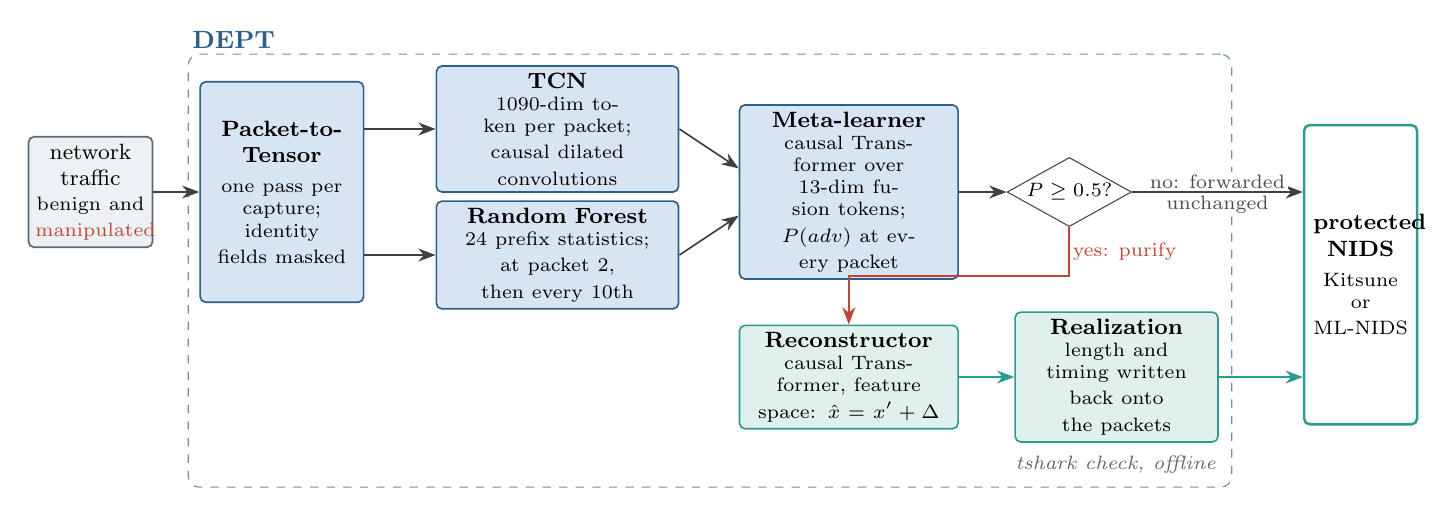
\begin{tikzpicture}[
    font=\footnotesize, >={Stealth[length=2.2mm]},
    blk/.style={draw=dblue, fill=dbluefill, rounded corners=2pt, align=center,
      inner sep=2.5pt, line width=0.6pt},
    pur/.style={draw=dteal, fill=dtealfill, rounded corners=2pt, align=center,
      inner sep=2.5pt, line width=0.6pt},
    neu/.style={draw=dgrey, fill=dgreyfill, rounded corners=2pt, align=center,
      inner sep=2.5pt, line width=0.6pt},
    arr/.style={->, line width=0.6pt, draw=black!75},
    lab/.style={font=\scriptsize, text=black!70, align=center, inner sep=1pt},
  ]
  % ---- input and pipeline
  \node[neu, text width=14mm, minimum height=13mm] (in) at (0.82,0)
    {network\\traffic\\[1pt]{\scriptsize benign and\\\textcolor{dred}{manipulated}}};
  \node[blk, text width=19mm, minimum height=28mm] (p2t) at (3.25,0)
    {\textbf{Packet-to-}\\\textbf{Tensor}\\[3pt]{\scriptsize one pass per\\capture; identity\\fields masked}};
  % ---- base learners
  \node[blk, text width=29mm, minimum height=12mm] (tcn) at (6.75,0.8)
    {\textbf{TCN}\\{\scriptsize 1090-dim token per packet;\\causal dilated convolutions}};
  \node[blk, text width=29mm, minimum height=12mm] (rf) at (6.75,-0.8)
    {\textbf{Random Forest}\\{\scriptsize 24 prefix statistics;\\at packet 2, then every 10th}};
  % ---- meta-learner and gate
  \node[blk, text width=26mm, minimum height=16mm] (meta) at (10.45,0)
    {\textbf{Meta-learner}\\{\scriptsize causal Transformer over\\13-dim fusion tokens;\\$P(\text{adv})$ at every packet}};
  \node[draw=black!70, fill=white, diamond, aspect=1.8, inner sep=0.5pt,
        font=\scriptsize] (gate) at (13.25,0) {$P \geq 0.5$?};
  % ---- purification
  \node[pur, text width=26mm, minimum height=12mm] (rec) at (10.45,-2.35)
    {\textbf{Reconstructor}\\{\scriptsize causal Transformer, feature\\space: $\hat{x} = x' + \Delta$}};
  \node[pur, text width=24mm, minimum height=12mm] (real) at (13.85,-2.35)
    {\textbf{Realization}\\{\scriptsize length and timing written\\back onto the packets}};
  \node[lab, text=black!60, below=1.2mm of real.south] (tshark)
    {\textit{tshark check, offline}};
  % ---- protected NIDS
  \node[draw=dteal, fill=white, rounded corners=2pt, line width=0.9pt,
        align=center, text width=12mm, minimum height=38mm] (nids) at (16.95,-1.05)
    {\textbf{protected}\\\textbf{NIDS}\\[3pt]{\scriptsize Kitsune or\\ML-NIDS}};
  % ---- DEPT frame
  \begin{scope}[on background layer]
    \node[draw=dblue!70, dashed, rounded corners=4pt, inner sep=4pt,
          fit=(p2t)(tcn)(rf)(meta)(gate)(rec)(real)(tshark)] (dept) {};
  \end{scope}
  \node[anchor=south west, font=\small\bfseries, text=dblue, inner sep=1.5pt]
    at (dept.north west) {DEPT};
  % ---- arrows
  \draw[arr] (in) -- (p2t);
  \draw[arr] (p2t.east |- tcn.west) -- (tcn.west);
  \draw[arr] (p2t.east |- rf.west) -- (rf.west);
  \draw[arr] (tcn.east) -- (meta.west |- 0,0.3);
  \draw[arr] (rf.east) -- (meta.west |- 0,-0.3);
  \draw[arr] (meta) -- (gate);
  \draw[arr] (gate.east) -- node[lab, above, pos=0.5, fill=white] {no: forwarded}
    node[lab, below, pos=0.5, fill=white] {unchanged} (nids.west |- gate.east);
  \draw[arr, draw=dred] (gate.south) -- node[lab, right, text=dred]
    {yes: purify} ++(0,-0.62) -| (rec.north);
  \draw[arr, draw=dteal] (rec) -- (real);
  \draw[arr, draw=dteal] (real.east) -- (nids.west |- real.east);
\end{tikzpicture}
\caption{DEPT in front of a protected NIDS. The packet-to-tensor pipeline
derives two views of each flow: bit-level packet tokens for the TCN and prefix
statistics for the Random Forest. The meta-learner fuses the two prediction
streams into a verdict at every packet. Unflagged flows pass unchanged; flagged
flows are corrected by the reconstructor and realized back into packets, so the
NIDS receives traffic, not tensors.}
\Description{A left-to-right diagram. Network traffic enters the
Packet-to-Tensor pipeline, which feeds per-packet tokens to a TCN and prefix
statistics to a Random Forest. Their dense and sparse logit streams enter the
meta-learner, followed by a threshold decision. Flows below the threshold go
directly to the protected NIDS. Flows above it go to the reconstructor and
then to the realization step, whose packets go to the protected NIDS. A note
says the tshark compliance check runs offline.}
\label{fig:arch}
\end{figure*}

\subsection{Overview}

\Cref{fig:arch} shows the architecture. A packet-to-tensor pipeline derives two
views of each flow: a dense stream of masked bit-level tokens, one per packet,
and a sparse stream of statistics over the flow's prefix. The TCN reads the
dense stream and emits a logit at every packet, from the first one; the Random
Forest reads the sparse stream and emits a logit at packet~2 and then every
tenth packet. A per-packet \emph{fusion token} joins the two prediction streams,
and the meta-learner, a small causal Transformer, turns it into a per-packet
probability that the flow is adversarial. Flows that never cross the threshold
are forwarded unchanged, so unflagged traffic pays for detection but not for
purification. Flagged flows go to the \emph{reconstructor}, which corrects them
in feature space, and a \emph{realization} step writes the correction onto the
packets. All components are trained offline in dependency order: the two base
learners on the training split, the meta-learner on the validation split, and
the reconstructor on matched pairs of adversarial and clean flows.

\subsection{Corpus and Traffic Representation}\label{sec:corpus}

\paragraph{Corpus} The corpus pairs ten traffic sources with their TANTGen
counterparts: the Mirai botnet and SSDP flood captures of
Kitsune~\cite{mirsky2018kitsune}; the DDoS, port scan and FTP/SSH brute-force
captures of CIC-IDS2017~\cite{cicids2017}; and the NTP, DNS, SSDP, SYN and LDAP
reflection and amplification floods of
CIC-DDoS-2019~\cite{sharafaldin2019cicddos}. These floods offer no clean time
window to filter on, so each is truncated to its first million packets, the
scale at which TANTGen caps its own input. TANTGen produced one variant per perturbation mode, giving 30 adversarial source--mode
combinations; tensorized, the 40 sources hold $8{,}624{,}958$ flows and
$61{,}516{,}406$ packets.

\paragraph{Labels} Every flow of the raw datasets is labelled \emph{benign},
including their native attacks, and every TANTGen flow \emph{adversarial}.
Detecting a flood or a scan is the protected NIDS's task; DEPT must recognize
whether the generator touched the flow. In the rest of this paper,
\emph{benign} therefore means \emph{unmanipulated}. The cost of this convention
is that, where TANTGen barely changes a flow, the two classes are nearly
indistinguishable for any detector.

\paragraph{Packet tokens} Each capture is processed in one pass, grouping
packets into flows by their five-tuple and keeping them in time order.
Following nPrint~\cite{holland2021nprint}, the IPv4, TCP, UDP and ICMP headers
of each packet are encoded bit by bit into $1{,}088$ tri-state cells ($1$ or $0$
for a set or unset bit, $-1$ for a layer absent from the packet), to which we
append the z-scored inter-packet arrival time (IPAT) and a direction bit,
giving a $1{,}090$-dimensional token. The $144$ bits that identify hosts and
ports (IP addresses, transport ports and IP identification) are set to zero, so
that a model cannot score well by memorizing the hosts of a
capture~\cite{arp2022dos} and must rely on behaviour, such as sizing and timing.

\paragraph{Prefix statistics} For the Random Forest, the same pass measures six
quantities on the packets themselves: IPAT, packet size, payload length,
payload entropy, TCP flags and direction. Each is summarized by its mean,
standard deviation, minimum and maximum over the prefix seen so far, a
$24$-dimensional vector updated incrementally (Welford's algorithm and running
extremes), so the cost per packet is constant. Checkpoints fire at packet~2 and
then every tenth packet. The early checkpoint exists because some attacks are
very short: a port scan averages about two packets per flow. Since nPrint
encodes headers only, the payload entropy that the forest uses is invisible to
the TCN, which adds to the diversity between the two learners.

\paragraph{Split and class balance} All models share one $70/15/15$ split into
training, validation and test sets, made at flow level (every token, checkpoint
or pair of a flow falls on the same side) and stratified by source. Their results are
therefore directly comparable, and the meta-learner is never evaluated on flows
that a base learner trained on. Because the reflection floods contribute far
more benign flows than the other sources, the benign pool is capped at three
flows per adversarial flow, and all losses use balanced class weights.

\subsection{Heterogeneous Detection Ensemble}\label{sec:ensemble}

\paragraph{Random Forest} At every checkpoint, the RF~\cite{breiman2001random}
decides whether the prefix statistics look manipulated. Forests are strong and
cheap on small tabular inputs, and their decision function is piecewise
constant, with no informative gradient for an attacker to follow. A grid search
on the validation split selected $200$ trees of maximum depth $20$ with at least
five samples per leaf, the most regularized setting of the grid.

\paragraph{TCN} The TCN~\cite{bai2018empirical} reads the token stream and emits
a logit at every packet. It has three residual blocks of $128$ channels, each
with two causal convolutions of kernel size $k=3$, with dilations $1$, $2$ and
$4$ (about $0.8$M parameters). Its receptive field is
$1 + 2(k-1)(1+2+4) = 29$ packets, so a verdict depends on the current packet and
the $28$ before it, and never on future packets. The per-packet cross-entropy is
averaged within each flow before averaging across flows, so that a long flood
does not drown two-packet scans in the gradient.

\begin{figure}[t]
  \centering
  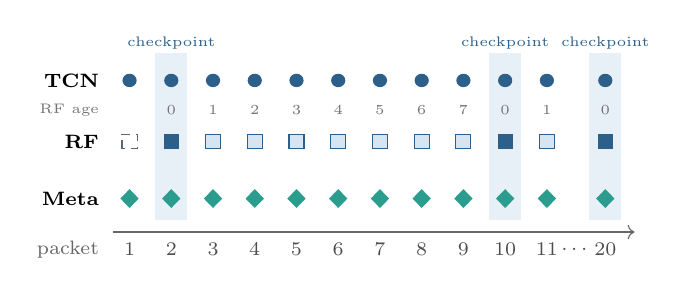
\begin{tikzpicture}[font=\scriptsize, x=5.3mm, y=5mm]
    % packets 1--11 are drawn at x = 1..11 and packet 20 at x = 12.4
    \foreach \x in {2,10,12.4} {
      \fill[dbluefill!60] (\x-0.38,-0.55) rectangle (\x+0.38,3.7);
      \node[text=dblue, font=\tiny] at (\x,3.95) {checkpoint};
    }
    % row labels
    \node[anchor=east, align=right] at (0.5,3.0) {\textbf{TCN}};
    \node[anchor=east, text=black!55, font=\tiny] at (0.5,2.25) {RF age};
    \node[anchor=east, align=right] at (0.5,1.45) {\textbf{RF}};
    \node[anchor=east, align=right] at (0.5,0) {\textbf{Meta}};
    \node[anchor=east, text=black!60] at (0.5,-1.3) {packet};
    % TCN: a logit at every packet
    \foreach \x in {1,...,11,12.4}
      \fill[dblue] (\x,3.0) circle (0.17);
    % RF: none before packet 2, fresh at checkpoints, carried forward between
    \draw[dgrey, densely dashed, line width=0.4pt]
      (0.82,1.27) rectangle (1.18,1.63);
    \foreach \x/\a in {2/0,3/1,4/2,5/3,6/4,7/5,8/6,9/7,10/0,11/1,12.4/0}
      \node[text=black!55, font=\tiny] at (\x,2.25) {\a};
    \foreach \x in {3,...,9,11}
      \draw[dblue, fill=dbluefill, line width=0.4pt]
        (\x-0.18,1.27) rectangle (\x+0.18,1.63);
    \foreach \x in {2,10,12.4}
      \fill[dblue] (\x-0.18,1.27) rectangle (\x+0.18,1.63);
    % meta-learner: a fused verdict at every packet
    \foreach \x in {1,...,11,12.4}
      \fill[dteal] (\x,0.24) -- (\x+0.22,0) -- (\x,-0.24) -- (\x-0.22,0) -- cycle;
    % packet axis
    \draw[->, black!60] (0.6,-0.85) -- (13.1,-0.85);
    \foreach \x in {1,...,11}
      \node[text=black!70] at (\x,-1.3) {\x};
    \node[text=black!70] at (11.7,-1.3) {\dots};
    \node[text=black!70] at (12.4,-1.3) {20};
  \end{tikzpicture}
  \caption{Prediction cadence over the first packets of a flow. The TCN emits a
  logit at every packet; the RF emits one at packet~2 and every tenth packet
  (dark squares) and its last logit is carried forward (light squares), with its
  age in packets given to the meta-learner, which fuses both at every packet.}
  \Description{A timeline of packets 1 to 11 and 20. The TCN row has a dot at
  every packet. The Random Forest row has an empty dashed square at packet 1,
  dark squares at the checkpoints at packets 2, 10 and 20, and light squares at
  the other packets, with an age counter that resets to 0 at each checkpoint.
  The meta-learner row has a diamond at every packet.}
  \label{fig:cadence}
\end{figure}

\paragraph{Meta-learner} The difficulty in fusing the two learners is
asynchrony (\Cref{fig:cadence}): at most packets the forest has no fresh
opinion, and before packet~2 it has none, so a fixed rule such as averaging is
not even defined everywhere.
The meta-learner is a decoder-only Transformer~\cite{vaswani2017attention} (two
causal blocks, four heads, $d_{\text{model}}=64$, about $68$k parameters) over a
$13$-dimensional fusion token: the RF logit carried forward from the last
checkpoint (a learnable placeholder before packet~2), the TCN logit, the number
of packets since the last RF refresh, a flag marking a refresh at this packet,
and a small summary of the packet (z-scored IPAT, direction, length and six TCP
flags). The full header representation is withheld on purpose, so that the
model combines its base learners instead of bypassing them. To avoid learning
the overfit confidence of the base learners~\cite{wolpert1992stacked}, it is
trained on the validation split, where their predictions are out-of-fold. Its
loss is the same balanced per-packet cross-entropy plus an auxiliary term
(weight $0.5$) that penalizes, at each packet, any shortfall of its confidence
in the true class against the better of the two base learners. A flow is
flagged the first time its probability $p_t$ crosses $0.5$.

\subsection{Purification and Realization}\label{sec:purifier}

\paragraph{Reconstructor} The reconstructor is a causal Transformer denoiser
over the token sequence (three layers, four heads, $d_{\text{model}}=128$,
about $678$k parameters). Given an adversarial flow $x' = (x'_1,\dots,x'_L)$, it
predicts a residual correction for every token and outputs
\begin{equation}
  \hat{x}_t = x'_t + \Delta_t, \qquad \Delta_t = g_\theta(x'_1,\dots,x'_t),
  \label{eq:residual}
\end{equation}
so each correction depends only on the current and earlier packets. TANTGen
moves only a few of the $1{,}090$ dimensions of a token, so with a residual
head the identity ($\Delta \approx 0$) is the easy default, and the roughly
$1{,}050$ untouched header bits are preserved. The model is not autoregressive:
it corrects all positions in one pass, and the causal mask is there for
streaming. Unlike generative purifiers, it does not model the distribution of
benign traffic; it regresses the correction directly.

\paragraph{Training on matched pairs} TANTGen keeps each flow's five-tuple, so
every adversarial flow can be aligned with the clean flow it was derived from.
The reconstructor is trained on these (adversarial $\rightarrow$ clean) pairs,
without single-packet pairs, using a smooth-L1 loss
between $\hat{x}$ and the clean flow, averaged within each flow. The loss
weights all $1{,}090$ dimensions equally, so the training signal holds no hint
of where the perturbation is: the model has to find which dimensions were
tampered with. This keeps the feature-space stage attack-agnostic.

\paragraph{Realization} Packets cannot be rebuilt from the purified tensors
alone, since nPrint encodes headers only and the identity fields are masked.
Realization therefore works by overlay: each original packet keeps its identity
and payload content, and only the two quantities purification may change are
written back. The purified IPv4 total length, decoded from its 16 header bits,
is applied by trimming the payload, the inverse of TANTGen's padding, and the
purified IPAT is de-normalized and applied to the packet's timestamp. Packets are
then re-serialized with scapy, which recomputes checksums and length fields. The
price is that the deployed pipeline is not attack-agnostic end to end: a flow
manipulated in another field, such as the time-to-live (TTL), would be flagged and denoised in
feature space, but would reach the NIDS unrepaired. Every realized packet is
finally checked with the \texttt{tshark} dissector; this check is a measurement
made offline, not a step on the inference path. A size edit on an
application-layer (L7) text protocol, such as the SSDP \texttt{M-SEARCH} messages
of one source, breaks the L7 grammar even when the IP and UDP fields stay valid.
Such packets cannot be realized faithfully by overlay and are reported
separately.

\subsection{Implementation}\label{sec:impl}

\begin{table}[t]
  \caption{Configuration of the four learned components. A step is a checkpoint
  for the RF and a packet for the three sequence models.}
  \label{tab:config}
  \footnotesize
  \setlength{\tabcolsep}{3.5pt}
  \begin{tabular}{@{}lcccc@{}}
    \toprule
    & RF & TCN & Meta-learner & Reconstructor \\
    \midrule
    Input per step & $24$ & $1{,}090$ & $13$ & $1{,}090$ \\
    Structure & $200$ trees & $3$ blocks & $2$ layers & $3$ layers \\
    Width & depth $20$ & $128$ channels & $d=64$, $4$ heads & $d=128$, $4$ heads \\
    Regularization & min.\ leaf $5$ & dropout $0.15$ & dropout $0.1$ & dropout $0.1$ \\
    Parameters & --- & $805{,}762$ & $67{,}971$ & $677{,}698$ \\
    Loss & Gini & balanced CE & bal.\ CE $+$ aux. & smooth-L1 \\
    Learning rate & --- & $10^{-3}$ & $3\cdot10^{-4}$ & $3\cdot10^{-4}$ \\
    Batch size & --- & $32$ & $128$ & $32$ \\
    Selection & val.\ macro-$F_1$ & val.\ macro-$F_1$ & AUROC@10 & val.\ loss \\
    \bottomrule
  \end{tabular}
\end{table}

\Cref{tab:config} summarizes the learned components; the sequence models are
trained with AdamW for at most $20$ epochs, with early stopping on the
selection criterion of the table. DEPT is written in Python, with PyTorch for the three sequence models,
scikit-learn for the forest, and a native reimplementation of the nPrint
encoding on top of scapy, which also performs realization; \texttt{tshark},
\texttt{editcap} and \texttt{tcpdump} handle dissection, time filtering and
packet capping. All experiments ran on one server with two Intel Xeon Gold 5320
CPUs, 160\,GB of RAM and two NVIDIA RTX 6000 Ada GPUs. Generating the 30
adversarial captures took $26.7$\,h and tensorization $11.2$\,h; training took
$2.7$\,h for the RF (with its grid search), $24.7$\,h for the TCN, $3.4$\,h for
the meta-learner and $10$\,h for the reconstructor.

%% ============================================================================
\section{Evaluation}\label{sec:evaluation}

\subsection{Research Questions and Setup}

The evaluation answers two research questions. \textbf{RQ1} (ensemble
robustness): does heterogeneous stacking measurably raise the cost of a
transferable, gradient-guided evasion attack, compared with a
single-architecture model? \textbf{RQ2} (purification): does the reconstructor
bring a flagged flow back towards its clean form, closing the detection gap
seen by the protected NIDS, while emitting realizable packets? Before them, we
report how early and how well DEPT detects manipulation. The latency of the full
pipeline is not evaluated in this work.

\paragraph{Test data} The held-out test split has $1{,}293{,}737$ flows, of which
$83.7\%$ are adversarial, because the reflection floods dominate; the RF, whose
first checkpoint is packet~2, does not score the $6{,}179$ single-packet flows.
Because of this base rate, the models are compared with the area under the ROC
curve (AUROC) and on the streaming axis rather than on accuracy. Of the $7{,}217{,}272$ adversarial
flows, $2{,}566{,}489$ have a matched clean counterpart; the shared split uses
$1{,}796{,}542$ pairs for training and holds out $384{,}963$ test pairs.

\paragraph{Metrics} AUROC@$t$ is the AUROC computed with each flow's
prediction after its first $t$ packets. The earliest detection
packet (EDP) is the median packet at which a flow's score first crosses $0.5$,
and the detection rate is the fraction of adversarial flows that ever cross it.
For purification, the reconstruction MSE is computed on the dimensions TANTGen
perturbed, between a flow and its true clean counterpart; as cells are ternary,
$1.0$ is the typical cost of a flipped bit. The main purification metrics are
measured through an \emph{independent} NIDS: the traffic of each attack is
scored by the detector TANTGen calibrated that attack against, Kitsune
(KitNET with AfterImage) for the two Kitsune sources and TANTGen's per-attack
CICFlowMeter flow classifiers (ML-NIDS) for the eight CIC attacks, so no DEPT
component grades itself. With $D$ the detection rate of that NIDS, we report the
attack success rate $\text{ASR} = 1 - D$ and the restoration ratio
\begin{equation}
  \rho = \frac{D_{\text{pur}} - D_{\text{adv}}}{D_{\text{clean}} - D_{\text{adv}}},
  \label{eq:rho}
\end{equation}
the fraction of the detection lost to TANTGen that purification recovers. A
gain measured through DEPT's own TCN is kept only as a sanity check, since it
is circular. Protocol compliance is the fraction of realized packets that
\texttt{tshark} parses without a malformed-packet error.

\subsection{Detection}\label{sec:eval-detect}

\begin{table}[t]
  \caption{Streaming detection on the held-out test flows. AUROC@$t$ uses each
  flow's prediction after $t$ packets; EDP is the median packet of first
  detection; the detection rate counts adversarial flows ever flagged.}
  \label{tab:streaming}
  \footnotesize
  \begin{tabular}{@{}lccc@{}}
    \toprule
    Metric & RF & TCN & Meta-learner \\
    \midrule
    First verdict at & packet 2 & \textbf{packet 1} & \textbf{packet 1} \\
    AUROC@1 & --- & 0.8191 & \textbf{0.8373} \\
    AUROC@2 & \textbf{0.9805} & 0.8225 & 0.9099 \\
    AUROC@5 & \textbf{0.9805} & 0.8375 & 0.9319 \\
    AUROC@10 & \textbf{0.9813} & 0.8371 & 0.9323 \\
    AUROC@max & \textbf{0.9813} & 0.8386 & 0.9334 \\
    EDP (median) & 2 & \textbf{1} & \textbf{1} \\
    Detection rate & \textbf{88.99\%} & 78.40\% & 77.69\% \\
    \bottomrule
  \end{tabular}
\end{table}

\Cref{tab:streaming} compares the three models on the streaming axis. The
result is not the one the design predicted: the Random Forest alone is the
strongest model from packet~2 on, at $0.9805$ at its first checkpoint and
$0.9813$ at the end, against $0.9099$--$0.9334$ for the meta-learner and
$0.8225$--$0.8386$ for the TCN. The fusion still gives three things. At
packet~1, where the forest is silent, the meta-learner has the best verdict
available ($0.8373$ against the TCN's $0.8191$). From packet~2 on, it beats the
TCN by $8.7$ to $9.5$ AUROC points. And it is the hardest of the three models to
evade (\Cref{sec:eval-rq1}). At the $0.5$ threshold all models favour precision:
the meta-learner flags only $1{,}115$ of the $211{,}151$ benign test flows, at an
adversarial recall of $0.708$.

\begin{table*}[t]
  \caption{End-of-flow AUROC per source and perturbation mode, against benign
  flows of the same source. $n_{\text{adv}}$ is the number of adversarial test
  flows per mode (on \src{mirai}, the RF scores $867$ of the $1{,}957$, as many
  flows end before packet~2). Values below $0.55$ are marked with $\dagger$.}
  \label{tab:persource}
  \footnotesize
  \setlength{\tabcolsep}{5pt}
  \begin{tabular}{@{}lr ccc ccc ccc@{}}
    \toprule
    & & \multicolumn{3}{c}{\dmode{both}} & \multicolumn{3}{c}{\dmode{iat}} & \multicolumn{3}{c}{\dmode{size}} \\
    \cmidrule(lr){3-5}\cmidrule(lr){6-8}\cmidrule(lr){9-11}
    Source (dataset) & $n_{\text{adv}}$ & RF & TCN & Meta & RF & TCN & Meta & RF & TCN & Meta \\
    \midrule
    \src{brute\_force} (CIC-IDS2017) & $1{,}045$ & 0.974 & 0.978 & 0.981 & 0.974 & 0.978 & 0.979 & 0.990 & 0.978 & 0.989 \\
    \src{ddos} (CIC-IDS2017) & $5{,}781$ & 1.000 & 1.000 & 1.000 & 0.999 & 0.924 & 0.967 & 1.000 & 1.000 & 1.000 \\
    \src{portscan} (CIC-IDS2017) & $23{,}800$ & 1.000 & 0.997 & 0.998 & 1.000 & 0.652 & 0.757 & 0.998 & 0.997 & 0.997 \\
    \src{mirai} (Kitsune) & $1{,}957$ & 0.926 & 0.680 & 0.724 & 0.919 & 0.680 & 0.719 & 0.829 & 0.723 & 0.734 \\
    \src{ssdp\_flood} (Kitsune) & $9{,}830$ & 1.000 & 0.999 & 1.000 & 1.000 & 1.000 & 1.000 & 1.000 & 0.999 & 1.000 \\
    \src{syn\_ddos} (CIC-DDoS-2019) & $200{,}483$ & 1.000 & 1.000 & 1.000 & 1.000 & 0.647 & 0.806 & 1.000 & 1.000 & 1.000 \\
    \src{dns\_ddos} (CIC-DDoS-2019) & $1{,}019$ & 0.999 & 0.552 & 1.000 & 0.999 & 0.547$\dagger$ & 1.000 & 0.258$\dagger$ & 0.531$\dagger$ & 0.443$\dagger$ \\
    \src{ldap\_ddos} (CIC-DDoS-2019) & $74{,}710$ & 1.000 & 0.500$\dagger$ & 1.000 & 1.000 & 0.500$\dagger$ & 1.000 & 0.476$\dagger$ & 0.501$\dagger$ & 0.476$\dagger$ \\
    \src{ntp\_ddos} (CIC-DDoS-2019) & $2{,}103$ & 0.999 & 0.514$\dagger$ & 0.654 & 0.999 & 0.497$\dagger$ & 0.653 & 0.213$\dagger$ & 0.494$\dagger$ & 0.493$\dagger$ \\
    \src{ssdp\_ddos} (CIC-DDoS-2019) & $40{,}446$ & 1.000 & 0.499$\dagger$ & 0.927 & 1.000 & 0.502$\dagger$ & 0.927 & 0.409$\dagger$ & 0.497$\dagger$ & 0.497$\dagger$ \\
    \bottomrule
  \end{tabular}
\end{table*}

The aggregate hides large differences between sources. \Cref{tab:persource}
measures each source--mode combination against benign flows of the same
source, which is DEPT's task as posed and the strictest view we record. Most
combinations are solved: $21$ of the $30$ reach at least $0.99$ for the RF, and
$13$ for the meta-learner. Three patterns stand out. First, timing-only edits
are hard for the TCN and easy for the forest (\src{portscan} \dmode{iat}:
$0.652$ against $1.000$; \src{syn\_ddos} \dmode{iat}: $0.647$ against $1.000$):
aggregated timing statistics capture a pure timing shift that the per-packet
sequence does not, which is the complementarity the ensemble was built on.
Second, the TCN is blind on the four reflection floods, at $0.494$--$0.552$ in
every mode: their flows are one- or two-packet UDP exchanges, and a receptive
field of $29$ packets has nothing to convolve over. Third, the \dmode{size}
variants of the DNS, NTP, SSDP and LDAP floods are at or below chance for every
model; below chance, a TANTGen flow looks more like generic benign traffic than
the flood's own unedited flows do (\Cref{sec:discussion}). The \src{mirai}
source fails differently: no model solves it in any mode, but none falls below
chance either.

The meta-learner also follows its stronger base learner only in part: on
\src{ntp\_ddos} \dmode{both} and \dmode{iat} it reaches $0.653$--$0.654$ where
the forest reaches $0.999$, and on \src{ssdp\_ddos} $0.927$ against $1.000$. The
likely cause is that the RF logit enters the fusion token as a single feature
refreshed only at checkpoints, while the TCN logit changes at every packet, so
attention under-weights the intermittent evidence. The auxiliary loss falls from
$0.0267$ to $0.0177$ during training, moving the meta-learner towards its better
base learner, but does not close this gap. Perhaps longer training would.

\subsection{Robustness to a Gradient-guided Attacker (RQ1)}\label{sec:eval-rq1}

\paragraph{Attack} TANTGen exercises no gradient path into DEPT, so it cannot
answer RQ1. The second adversary of \Cref{sec:threat} crafts one perturbation
against the TCN with PGD~\cite{madry2018towards} and replays it, unchanged,
through the TCN, the RF and the fused stack; re-optimizing it for each target
would no longer measure transfer. The perturbation adds padding (random bytes)
and delay to each packet, on top of TANTGen's own, under five per-packet budgets
from $8$ bytes and $10\,\mu$s to $1{,}460$ bytes and $100$\,ms. Three controls
guard against a weak attack~\cite{carlini2019evaluating,tramer2020adaptive}: a
random search with the same feasible set and number of queries, a cross-check
with the parameter-free AutoPGD~\cite{croce2020reliable} of the ART
library~\cite{nicolae2018adversarial}, which agrees with our PGD, and a reported
attacker that takes the best of PGD and random search for each flow. We sample
$9{,}000$ test flows ($300$ per source--mode combination), set each target's
threshold at a matched $5\%$ false-positive rate on benign traffic, and measure
ASR only over the flows each target detects without perturbation ($7{,}510$ for
the RF, $3{,}374$ for the TCN and $7{,}597$ for the stack). Since the budgets are
nested, a larger budget can always spend less.

\begin{figure}[t]
  \centering
  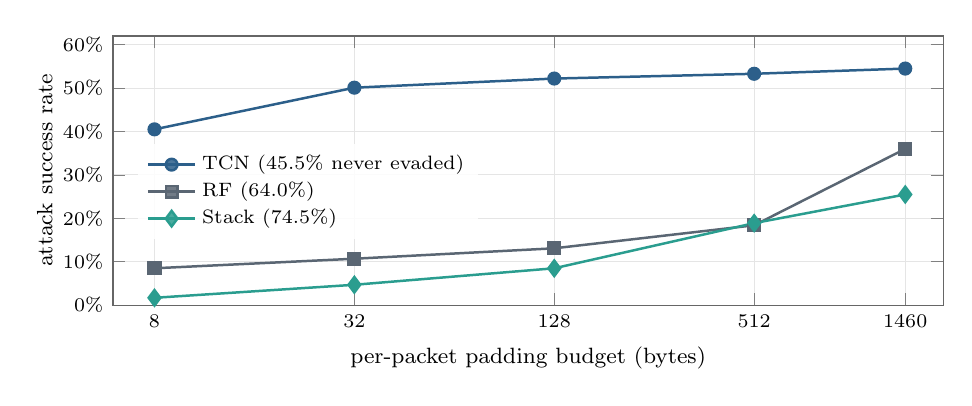
\begin{tikzpicture}
    \begin{axis}[
        width=\columnwidth, height=50mm,
        xmode=log, log basis x=2,
        xmin=6, xmax=1900,
        xtick={8,32,128,512,1460}, xticklabels={8,32,128,512,1460},
        ymin=0, ymax=62, ytick={0,10,20,30,40,50,60},
        yticklabel={\pgfmathprintnumber{\tick}\%},
        xlabel={per-packet padding budget (bytes)},
        ylabel={attack success rate},
        tick label style={font=\scriptsize}, label style={font=\footnotesize},
        ylabel shift=-3pt,
        grid=major, grid style={draw=black!10},
        axis line style={draw=black!60},
        legend style={font=\scriptsize, draw=none, fill=white, fill opacity=0.85,
          text opacity=1, at={(0.03,0.6)}, anchor=north west, row sep=-1pt},
        legend cell align=left,
        every axis plot/.append style={line width=0.9pt, mark size=2.1pt},
      ]
      \addplot[color=dblue, mark=*] coordinates
        {(8,40.5) (32,50.1) (128,52.2) (512,53.3) (1460,54.5)};
      \addlegendentry{TCN (45.5\% never evaded)}
      \addplot[color=dgrey, mark=square*] coordinates
        {(8,8.5) (32,10.7) (128,13.1) (512,18.4) (1460,36.0)};
      \addlegendentry{RF (64.0\%)}
      \addplot[color=dteal, mark=diamond*, mark size=2.8pt] coordinates
        {(8,1.7) (32,4.7) (128,8.5) (512,18.9) (1460,25.5)};
      \addlegendentry{Stack (74.5\%)}
    \end{axis}
  \end{tikzpicture}
  \caption{Attack success of one perturbation crafted with the TCN's gradients
  and replayed unchanged through each target, at a matched $5\%$
  false-positive rate. In parentheses: flows never evaded at any budget.}
  \Description{A line chart of attack success rate against the per-packet
  padding budget on a log scale from 8 to 1460 bytes. The TCN line rises from
  40.5 percent to 54.5 percent. The Random Forest line rises from 8.5 to 36.0
  percent. The stack line rises from 1.7 to 25.5 percent, stays below the
  forest except at 512 bytes, where both are near 18.5 percent.}
  \label{fig:rq1}
\end{figure}

\paragraph{Results} \Cref{fig:rq1} shows the outcome. The perturbation breaks
the TCN it was crafted against, transfers poorly to the forest, and the fused
stack is harder still: at $8$, $32$ and $128$ bytes per packet it concedes
$1.7\%$, $4.7\%$ and $8.5\%$ attack success, against $8.5\%$, $10.7\%$ and
$13.1\%$ for the RF and $40.5\%$ to $52.2\%$ for the TCN. Over the whole grid,
$74.5\%$ of the flows never evade the stack at any budget, against $64.0\%$ for
the RF and $45.5\%$ for the TCN, whose median evading flow needs only the
smallest budget. The ordering is not uniform: at $512$ bytes the stack and the
forest are level ($18.9\%$ and $18.4\%$), and the stack pulls ahead again at
$1{,}460$ bytes ($25.5\%$ against $36.0\%$). For scale, TANTGen's own padding
averages $29$ to $32$ bytes per packet on \src{portscan} \dmode{both} and
\src{mirai} \dmode{size}, where the stack concedes at most $8.5\%$, but $246$ to
$289$ bytes on the \dmode{size} variants of \src{ddos}, \src{ssdp\_flood} and
\src{portscan}, closer to the $512$-byte point.

The mechanism the design predicted is visible. When each base-learner slot of
the fusion token is given back its clean value, the share of the
meta-learner's verdict that moves with the forest goes from $0$ without attack,
where there is nothing to compensate, to between $0.53$ and $0.56$ at every
non-zero budget: the stack leans on the learner the attacker cannot
differentiate. Against the
TCN, random search slightlybeats PGD at every budget ($40.1\%$ against $37.2\%$ at
$8$ bytes), so what was measured is a search-based attacker that happens to have
a gradient; regardless, since both searches are crafted on the TCN, the conclusion that the
non-differentiable member raises the cost of evasion still holds.

\subsection{Purification (RQ2)}\label{sec:eval-purif}

\begin{table}[t]
  \caption{Purification on the $384{,}963$ held-out test pairs. The TCN row is
  circular and kept as a sanity check; compliance counts realizable packets only.}
  \label{tab:purif}
  \footnotesize
  \setlength{\tabcolsep}{4pt}
  \begin{tabular}{@{}lc@{}}
    \toprule
    Quantity & Value \\
    \midrule
    MSE on perturbed dimensions (adv.\ $\rightarrow$ purified) & $0.918 \rightarrow 0.054$ ($17.0\times$) \\
    TCN $P(\text{adv})$ (adv.\ $\rightarrow$ purified; clean) & $0.675 \rightarrow 0.428$; $0.421$ \\
    Independent NIDS detection (adv.\ $\rightarrow$ purified) & $0.781 \rightarrow 0.906$ \\
    Clean ceiling of the same NIDS & $0.980$ \\
    Restoration ratio $\rho$ & $\mathbf{63.0\%}$ \\
    \texttt{tshark} pass rate & $\mathbf{97.22\%}$ \\
    L7-text packets not realizable (reported apart) & $450{,}758$ \\
    \bottomrule
  \end{tabular}
\end{table}

\begin{table*}[t]
  \caption{Attack success rate (\%) of the protected NIDS per attack, over the
  three perturbation modes. Left: full realized streams through the gated
  pipeline, where only flows flagged by the meta-learner are purified; $\Delta$
  is the reduction in points. Right: held-out test pairs, with DEPT's
  reconstructor or the diffusion purifier of \citet{merzouk2024diffusion} applied
  to every flow. On the test pairs, Kitsune misses almost all traffic even when
  clean, so its two rows say little.}
  \label{tab:e2e}
  \footnotesize
  \setlength{\tabcolsep}{6pt}
  \begin{tabular}{@{}ll rrrr rrrr@{}}
    \toprule
    & & \multicolumn{4}{c}{Full streams, gated pipeline} & \multicolumn{4}{c}{Held-out test pairs, purifier only} \\
    \cmidrule(lr){3-6}\cmidrule(lr){7-10}
    Attack & NIDS & Clean & Before & After & $\Delta$ & Clean & No defense & Diffusion & DEPT \\
    \midrule
    \src{ddos}        & ML-NIDS & 7.8 & 61.6 & 23.4 & $+38.2$ & 21.0 & 68.4 & 89.3 & \textbf{35.7} \\
    \src{portscan}    & ML-NIDS & 0.1 & 66.1 & 34.2 & $+31.9$ & 0.2 & 66.1 & 83.6 & \textbf{34.3} \\
    \src{syn\_ddos}   & ML-NIDS & 0.1 & 4.7 & 0.0 & $+4.7$ & 0.2 & 4.7 & 39.1 & \textbf{0.0} \\
    \src{ntp\_ddos}   & ML-NIDS & 0.2 & 1.1 & 0.9 & $+0.2$ & 0.1 & 1.1 & 4.4 & 1.3 \\
    \src{ldap\_ddos}  & ML-NIDS & 0.0 & 0.0 & 0.0 & $0.0$ & 0.0 & 0.0 & 0.0 & 0.0 \\
    \src{ssdp\_ddos}  & ML-NIDS & 0.2 & 0.2 & 0.2 & $0.0$ & 1.4 & 1.4 & 1.5 & 1.5 \\
    \src{brute\_force}& ML-NIDS & 0.8 & 0.9 & 2.1 & $-1.2$ & 0.6 & 0.4 & 0.8 & 1.6 \\
    \src{dns\_ddos}   & ML-NIDS & 0.6 & 1.3 & 19.2 & $-17.9$ & 1.0 & 1.3 & 1.7 & 24.0 \\
    \src{mirai}       & Kitsune & 99.7 & 91.8 & 99.8 & $-8.0$ & 99.6 & 91.3 & 98.4 & 99.8 \\
    \src{ssdp\_flood} & Kitsune & 0.0 & 0.0 & 0.0 & $0.0$ & 99.8 & 99.9 & 100.0 & 99.9 \\
    \midrule
    \textbf{Overall} & & \textbf{1.9} & \textbf{21.1} & \textbf{11.6} & $\mathbf{+9.5}$ & \textbf{5.7} & \textbf{31.5} & \textbf{40.3} & \textbf{18.9} \\
    \bottomrule
  \end{tabular}
\end{table*}

\Cref{tab:purif} summarizes the reconstructor. The error on the perturbed
dimensions falls $17$-fold, and DEPT's own TCN scores purified flows almost
exactly like the true clean ones. The main result is measured through the
independent NIDS: over $370{,}700$ realized flows, purification raises
detection from $0.781$ to $0.906$, against a clean ceiling of $0.980$, which
recovers $63.0\%$ of the gap TANTGen opened. On the eight ML-NIDS sources the
move is from $0.808$ to $0.910$ against $0.987$, an average diluted by the
sources where detection was never lost. Of the realizable packets, $97.22\%$
parse without errors, and only two sources fall below $0.99$: \src{ddos} ($0.84$)
and \src{syn\_ddos} \dmode{iat} ($0.178$).

The per-source view shows four outcomes. \emph{(i)~Footprint erased and detection
restored}, where TANTGen's edits are structural: \src{ddos} \dmode{size} from
$0.005$ to $0.817$ (clean $0.828$), \src{ddos} \dmode{both} from $0.080$ to
$0.865$, \src{portscan} \dmode{both} from $0.011$ to $0.679$ and \src{portscan}
\dmode{size} from $0.013$ to $0.479$. \emph{(ii)~Nothing to undo}: on the
\dmode{both} and \dmode{iat} variants of the reflection floods, the footprint is
near zero before purification, and on the \dmode{size} variants of
\src{ldap\_ddos}, \src{ntp\_ddos} and \src{ssdp\_ddos} the adversarial tokens are
bit-identical to the clean ones, because the attack did not fire. \emph{(iii)~A
judge that cannot see the effect}: on \src{dns\_ddos} \dmode{size} the footprint
falls from $1.000$ to $0.302$, but DEPT's TCN is blind on that source; on
\src{ssdp\_flood} \dmode{size} it is almost erased ($1.000\rightarrow0.003$), but
no packet of that stream survives L7 realization, so the NIDS cannot score it.
\emph{(iv)~Harm where TANTGen did not evade}: \src{dns\_ddos} falls from $0.986$
to $0.762$ in \dmode{both} and from $0.993$ to $0.756$ in \dmode{iat}, and
\src{portscan} \dmode{iat} from $0.994$ to $0.811$. The denoiser moves these flows
towards the clean manifold, but there the attack's fingerprint and the clean
manifold were never far apart, so it removes signal the NIDS was still using.
The \src{mirai} source, whose flows are often very short, is where purification
works least well: on \dmode{size}, the footprint only falls from $1.569$ to
$0.973$.

\subsection{End-to-end Deployment and Comparison with a Diffusion Purifier}\label{sec:eval-e2e}


\paragraph{Deployment} We place the full gated pipeline in front of each
protected NIDS: the meta-learner flags flows, only flagged flows are purified,
and the rest pass unchanged. For every attack, three realized full streams are
scored through its NIDS: the clean attack (the NIDS working as intended), the
adversarial traffic (before DEPT) and the defended traffic (after DEPT). Over
$2{,}704{,}816$ scored flows, DEPT cuts attack success from $21.1\%$ to $11.6\%$
and recovers $49.3\%$ of the detection TANTGen had removed
(\Cref{tab:e2e}, left). The gain is large where TANTGen actually evaded: $38$
points on \src{ddos} and $32$ on \src{portscan}, and up to $67$ points on single
modes (\src{ddos} \dmode{size} and \src{portscan} \dmode{both}). Most other
attacks barely move, because TANTGen never evaded them. On some, the defense
makes things worse: \src{dns\_ddos} loses $22.5$ and $22.7$ points in
\dmode{both} and \dmode{iat}, \src{portscan} \dmode{iat} $18.2$, \src{ddos}
\dmode{iat} $12.2$ and \src{mirai} \dmode{size} $23.9$. On \src{mirai}
\dmode{size}, TANTGen's padding had raised Kitsune's detection from
$0.003$ to $0.242$; by undoing the padding, DEPT also undid that. By detector
family, the eight ML-NIDS attacks gain $9.9$ points over $2{,}622{,}023$ flows,
while the two Kitsune attacks lose $1.7$ points over $82{,}793$ flows, almost
all of it on \src{mirai} \dmode{size}.

The gate explains these losses. It flags almost all flood traffic, so flows the
NIDS was still catching get purified, except on the \dmode{size} variants of the
reflection floods, where it flags almost nothing ($0.0$ to $0.9\%$), the same
blind spot as in \Cref{tab:persource}. Purifying every flow
gives almost the same detection as the gated pipeline ($0.8831$ against
$0.8836$), so the gate does little work: it predicts whether a flow is
adversarial, while the pipeline needs to predict whether purifying the flow will
help. Because the defended streams also contain flows seen in training, we
repeated the measurement on held-out flows only: there the gated pipeline lowers
attack success from $31.4\%$ to $17.7\%$.

\paragraph{Comparison with a published purifier} To compare DEPT with the state
of the art, we replace its reconstructor by the diffusion-based purifier of
\citet{merzouk2024diffusion}, the only network purifier among the surveyed works
with public code, and keep the flows, the realization step and the NIDS. The
baseline keeps the authors' model and settings and learns from clean traffic
only; its amount of noise is chosen as in the original, but on validation
flows. Both
purifiers are scored on the held-out test pairs (\Cref{tab:e2e}, right). Attack
success is $31.5\%$ without defense, $18.9\%$ with DEPT and $40.3\%$ with the
diffusion purifier, and the order is the same on test flows whose original flow
appears in no training pair. The setup favours DEPT in two ways: DEPT learns from
matched TANTGen and clean flows and is tested against that same attacker, while
the baseline sees only clean traffic; and the baseline, designed for flow-level
features, had to be adapted to per-packet sizes and timings, and the timing
encoding chosen for it explains part of its losses on the floods whose
detection depends on timing.

On the five source--mode combinations where TANTGen lowered detection by more
than five points (\src{ddos} and \src{portscan} in \dmode{both} and \dmode{size},
and \src{syn\_ddos} \dmode{size}), DEPT recovers $63.5\%$ of the lost detection
and the diffusion purifier $0.5\%$, and no amount of noise did better on the
validation flows. A padded or delayed TANTGen flow still looks like realistic
traffic, so a purifier that only knows clean traffic has little reason to change
it. Elsewhere, both purifiers can lower detection. The diffusion purifier slows
down the floods whose detection depends on timing, raising attack success on
\src{syn\_ddos} from $4.7\%$ to $39.1\%$. DEPT is worse than it on the three
modes of \src{dns\_ddos}, on \src{brute\_force} \dmode{both} and on \src{mirai}
\dmode{size}, where the diffusion purifier barely changes the traffic.

\subsection{One Global Model or Ten Specialists?}\label{sec:eval-spec}

Detectors in the literature are often trained per attack. We therefore re-ran
the four model stages once per attack, with the same architectures, searches and
split protocol, and compared each specialist meta-learner with the global one on
the same flows. The two are indistinguishable on $13$ of the $30$ source--mode
combinations. Specialists win on timing: \src{ntp\_ddos} \dmode{both} and
\dmode{iat} ($+0.346$ and $+0.347$ AUROC), \src{syn\_ddos} \dmode{iat}
($+0.194$), \src{ssdp\_ddos} \dmode{both} and \dmode{iat} ($+0.073$) and
\src{portscan} \dmode{iat} ($+0.066$), since a model trained on one attack can
learn that source's own timing signature instead of averaging over nine unrelated
benign pools. The global model wins on the \dmode{size} variants of the
reflection floods, only by being less confidently wrong ($0.443$ against $0.192$
on \src{dns\_ddos}), and on \src{mirai} \dmode{both} and \dmode{iat} (by $0.035$
and $0.033$). The meta-learner below its own forest reappears in the specialists
(on \src{mirai}, $0.705$ against its RF's $0.889$), and the per-attack TCNs also
collapse on the reflection floods ($0.500$--$0.531$) while doing well on sources
with longer flows ($0.990$ on \src{ddos}), so neither problem comes from training
across sources. A
global model remains the right default: a specialist needs a router that names
the attack first, which is the very classification problem the detector exists
to solve. Specialists are worth considering for a known high-rate flood whose
evasion is expressed in timing.

%% ============================================================================
\section{Discussion and Limitations}\label{sec:discussion}

\paragraph{Research questions} RQ1 is answered positively: fusing a
non-differentiable learner with a differentiable one measurably raises the cost
of a transferable, gradient-guided evasion, with three limits. The ASR is
measured over the flows a target detects without perturbation, and the TCN
detects at most $2\%$ of the flows on seven of the ten sources, so its side of
the comparison rests on a minority of the corpus. On some combinations
(\src{ddos} and \src{portscan} in \dmode{both} and \dmode{size}, and
\src{ssdp\_flood} \dmode{size}), the forest and the stack are never evaded,
which only says that padding and delay cannot overcome that much model
confidence. And the attacker that was measured is, in effect, a search-based
one, even though the gradient-based one falls only shortly behind. RQ2 is answered
positively under a condition: purification restores detection where TANTGen
evaded, and is inert or harmful where it did not.

\paragraph{Size-perturbed reflection floods} On the \dmode{size} variants of the
DNS, NTP, SSDP and LDAP floods, every model scores at or below chance,
per-attack specialists included. On three of the four, every matched test pair
is bit-identical to its clean counterpart, so no detector can separate them; this
is a cost of the label convention. On \src{dns\_ddos}, the purifier cuts a full
footprint to under a third without moving DEPT's verdict, so the cause is likely the
representation: its $24$ prefix statistics and $1{,}088$ header bits cannot
express what separates such a flow from an unedited one. Since these floods
dominate the corpus, most aggregates average near-perfect and below-chance
sub-populations.

\paragraph{The gate and the fusion} Purification without an adequate gate
subtracts as well as adds, and the gate as built barely gates. The meta-learner,
in turn, is beaten by its own Random Forest from packet~2 on, although a stacking
ensemble should be no worse than its best base learner; the fusion still provides
the packet-1 verdict and the robustness of RQ1.

\paragraph{Validation and scope} The TCN-based purification gain is circular,
although no end-to-end claim rests on it. Each attack is judged by a single
NIDS, and on \src{mirai} that NIDS detects almost nothing even on the clean
attack. DEPT is compared with one published purifier, adapted to its
representation, and only against the attacker it was trained on. The purifier
corrects all $1{,}090$ dimensions without being told which the attacker moved,
but realization writes back only length and timing, so ``attack-agnostic''
describes the detector and the reconstructor, not the full deployed pipeline. The features
are limited to headers, timing, direction, and payload length and entropy, which
remain observable as more traffic is encrypted; payload content is never parsed,
which may be where the \src{dns\_ddos} blind spot lies. Finally, tensorization is
pure Python, slower than the native nPrint tool, and the latency study that
would settle the real-time budget of an inline defense remains to be done.

%% ============================================================================
\section{Conclusion and Future Work}\label{sec:conclusion}

DEPT is a streaming defense that detects realizable adversarial manipulation of
network traffic from the first packet, and purifies flagged flows back into
valid packets before they reach the protected NIDS. Evaluated against a
black-box, protocol-compliant generator over ten traffic sources and three
perturbation modes, its heterogeneous ensemble makes a gradient-guided evasion
measurably more expensive, and its reconstructor, judged by the detector each attack was
built to evade, recovers $63\%$ of the lost detection and nearly halves
end-to-end attack success, where a published diffusion purifier recovers almost
none.

As for the failures. A gate trained on whether purification
raises or lowers the protected detector's score, which the system already
computes, would turn the end-to-end losses into no-ops. Deriving the fields to
edit from the residual $\Delta$ and checking them against protocol constraints,
in the spirit of the SMT-checked perturbations of
PANTS~\cite{jin2025robustifying}, would extend realization beyond its two fixed
fields. The fusion should never fall below its best base learner, for instance
by letting the meta-learner fall back to the stronger opinion when the two
diverge. The comparison should be repeated with other purifiers and against
generators DEPT was not trained on. And payload content is the first place to
look for what separates a size-perturbed DNS flood flow from an unedited one.
Beyond these, a static defense is a fixed target: an adversary that probes it
long enough can map its blind spots. Casting the defense as a reinforcement
learning agent, rewarded by detection outcomes and retrained against an evolving
generator such as TANTGen~\cite{sutton2018reinforcement,nguyen2021deep}, is the
direction we consider most important.

\begin{acks}
We thank Inês Pissarra, whose work on TANTGen this work builds upon, for the
clarifications and for the materials that made it possible.
\end{acks}

\bibliographystyle{ACM-Reference-Format}
\bibliography{references}

\end{document}
\endinput
